\begin{minipage}{0.45\textwidth}
    \raggedright \large
    Introduce una \textbf{partizione} in $M$ classi di equivalenza $\mathcal{R}_1, \dots, \mathcal{R}_M$ su $Y$.
\end{minipage}
\hfill
\begin{minipage}{0.5\textwidth}
    \centering
    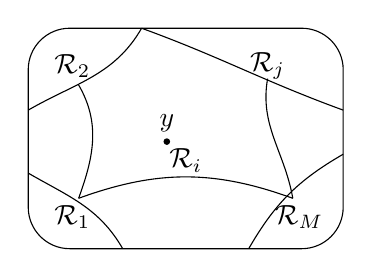
\begin{tikzpicture}[scale=0.8]
        \draw[rounded corners=15pt] (0,0) rectangle (5,3.5);

        \draw (0, 2.2) to[out=30, in=240] (1.8, 3.5);
        \draw (0, 1.2) to[out=-30, in=120] (1.5, 0);
        \draw (3.5, 0) to[out=60, in=210] (5, 1.5);
        \draw (1.8, 3.5) to[out=-20, in=160] (5, 2.2);

        % Linee interne per definire Ri
        \draw (0.8, 2.6) to[out=300, in=70] (0.8, 0.8);
        \draw (0.8, 0.8) to[out=20, in=160] (4.2, 0.8);
        \draw (4.2, 0.8) to[out=100, in=260] (3.8, 2.7);

        % Etichette delle regioni
        \node at (0.7, 2.9) {$\mathcal{R}_2$};
        \node at (0.7, 0.5) {$\mathcal{R}_1$};
        \node at (4.3, 0.5) {$\mathcal{R}_M$};
        \node at (3.8, 2.9) {$\mathcal{R}_j$};
        \node at (2.5, 1.4) {$\mathcal{R}_i$};

        \fill (2.2, 1.7) circle (1.5pt) node[above] {$\bm{y}$};

    \end{tikzpicture}
\end{minipage}